\documentclass[9pt,pdf,hyperref={unicode}]{beamer}
\beamertemplatenavigationsymbolsempty

\setbeamertemplate{blocks}[rounded=true, shadow=true]
\setbeamertemplate{footline}[page number]
\usepackage{multicol}

\usefonttheme{serif}

\usepackage[utf8]{inputenc}
\usepackage[english, russian]{babel}
\usepackage{amsmath,mathrsfs,mathtext}
\usepackage{graphicx, epsfig}
\usepackage{caption}
\usepackage{subfig}
\usepackage{amsmath, bm}

\usepackage{comment}
\usepackage{multirow}

\usepackage{tabularx}

\usepackage{tikz}

\DeclareMathOperator*{\argmin}{arg\,min}
\DeclareMathOperator*{\argmax}{arg\,max}

\makeatletter
\let\@@magyar@captionfix\relax
\makeatother

\usetheme{Warsaw}
\usecolortheme{sidebartab}
\definecolor{beamer@blendedblue}{RGB}{31,96,49}

\setbeamertemplate{enumerate items}[circle]

\setbeamersize{text margin left=1.5em, text margin right=1.5em}

\usepackage{ragged2e}

\usepackage{etoolbox}% http://ctan.org/pkg/etoolbox
\AtBeginEnvironment{figure}{\setcounter{subfigure}{0}}% Resets subfigure counter at start of figure environment

%----------------------------------------------------------------------------------------------------------
\title[\hbox to 56mm{истилляция и привилигированная информация \hfill\insertframenumber\,/\,\inserttotalframenumber}]
{Привилигированная информация и дистиляция моделей}
\author[А.\,В.~Грабовой]{\large \\Грабовой Андрей Валериевич}
\institute{\large
Московский физико-технический институт}

\date{\footnotesize{МФТИ, г. Долгопрудный}}
%----------------------------------------------------------------------------------------------------------

\begin{document}
%----------------------------------------------------------------------------------------------------------
\begin{frame}
\titlepage
\end{frame}

%----------------------------------------------------------------------------------------------------------
\begin{frame}{Вероятностная интерпретация дистилляции моделей}
\justifying
\textbf{Цель:} предложить вероятностную постановку задачи дистилляции моделей глубокого обучения на основе существующих методов дистилляции и привилегированного обучения.
%предложить метод построения ансамбля локально аппроксимирующих моделей для поиска окружностей на изображении.



~\\
\textbf{Задачи}

\begin{enumerate}
\justifying
	\item Поставить вероятностную задачу дистилляции для задачи классификации и регрессии.
	%Предложить метод поиска окружности при помощи линейной модели, для поиска нескольких окружностей предложить метод построения смеси локальных аппроксимирующих моделей.
	\item Провести теоретический анализ предложенной вероятностной постановки задачи для линейных моделей.
	%Предложить априорные распределения на параметры локальных моделей.
\end{enumerate}

~\\
\textbf{Исследуемая проблема}
\begin{enumerate}
\justifying
	\item Снижение размерности пространства параметров моделей глубокого обучения.
\end{enumerate}

~\\
\textbf{Метод решения}

	Предлагается поставить вероятностную постановку задачи дистилляции моделей глубокого обучения. В качестве базовой дистилляции предлагается использовать методы предложенные Дж. Хинтоном и В. Вапником.
	
\end{frame}

%----------------------------------------------------------------------------------------------------------
\begin{frame}{Список литературы}
\justifying
\begin{enumerate}
	\item \textit{Грабовой А.\,В., Стрижов В.\,В.} Анализ моделей привилегированного обучения и дистилляции // Автоматика и Телемеханика (на рассмотрении)
	\item \textit{Christopher Bishop}, Pattern Recognition and Machine Learning, 2016.
	\item \textit{Lopez-Paz D., Bottou L., Scholkopf B., Vapnik V.} Unifying Distillation and Privileged Information // In International Conference on Learning Representations. Puerto Rico, 2016.
	\item \textit{Hinton G., Vinyals O., Dean J.} Distilling the Knowledge in a Neural Network // NIPS Deep Learning and Representation Learning Workshop. 2015.
	\item \textit{Madala H., Ivakhnenko A.} Inductive Learning Algorithms for Complex Systems Modeling. Boca Raton: CRC Press Inc., 1994.
\end{enumerate}
\end{frame}

%----------------------------------------------------------------------------------------------------------

\begin{frame}{Введения}
\justifying
Когда возникает задача:
\begin{enumerate}
	\item изменение признакового описания объектов;
	\item использования информации из ``будущего'';
	\item уменьшение сложности модели;
	\item использования нескольких типо признаков.
\end{enumerate}

{\color{red} Сам слайд мне не нравится нужно переписать... Что сюда интересное можно придумать?}
\end{frame}
%----------------------------------------------------------------------------------------------------------
\begin{frame}{Необходимые понятия}
\justifying
\begin{definition}
\justifying
Дистилляция модели~--- уменьшение сложности модели путем выбора модели в множестве более простых моделей с использованием ответов более сложной модели.
\end{definition}

\begin{definition}
\justifying
Привилегированная информация~--- множество признаков, которые доступны только в момент выбора модели, но не в момент тестирования.
\end{definition}

\begin{definition}
\justifying
Учитель~--- фиксируемая модель, ответы которой используются при выборе модели ученика.
\end{definition}

\begin{definition}
\justifying
Ученик~--- модель, которая выбирается согласно какого-либо критерия.
\end{definition}

\end{frame}
%----------------------------------------------------------------------------------------------------------
\begin{frame}{Постановка задачи обучения с учителем}
\justifying
Задано:\\
\begin{enumerate}
	\item множество объектов~$\bm{\Omega}$, где $\left|\bm{\Omega}\right| = m$;
	\item множество объектов~$\bm{\Omega}^*$, где $\left|\bm{\Omega}^*\right| = m^*$;
	\item множество целевых переменных~$\mathbb{Y}$, причем~$\mathbf{y}_i = \mathbf{y}\bigr(\omega_i\bigr)$;
	\item отображение $\varphi:\bm{\Omega} \to \mathbb{R}^{n}$, обозначим $\mathbf{x}_i = \varphi(\omega_i)$;
	\item отображение $\varphi^*:\bm{\Omega}^* \to \mathbb{R}^{n^*}$, обозначим $\mathbf{x}^*_i = \varphi^*(\omega_i)$.
\end{enumerate}
Введем множество объектов, для которых известна привилигированя информация:
\[
\mathcal{I} = \{1 \leq i \leq m |~\text{для $i$-го объекта задана привилегированная информация}\},
\]
а множество индексов объектов, для которых не известна привилегированная информация, обозначим $\{1, \cdots, m\}\setminus \mathcal{I} = \bar{\mathcal{I}}$.

\end{frame}
%----------------------------------------------------------------------------------------------------------
\begin{frame}{Постановка задачи обучения с учителем}
\justifying
Пусть на множестве привилегированных признаков задана функция учителя~$\mathbf{f}\bigr(\mathbf{x}^*\bigr)$:
\[
\mathbf{f}:\mathbb{R}^{n^*} \to \mathbb{Y}^*.
\]
Заметим:
\begin{enumerate}
	\item множество $\mathbb{Y}^*=\mathbb{Y}$ для задачи регрессии;
	\item множество $\mathbb{Y}^*$ является единичным симплексом~$\mathcal{S}_K$ в пространстве размерности~$K$ для задачи классификации. 
\end{enumerate}
Для удобства введем обозначения:~$\mathbf{f}\bigr(\mathbf{X}^*\bigr)=\mathbf{S}$.

Требуется выбрать модель ученика~$\mathbf{g}\bigr(\mathbf{x}\bigr)$ из множества:
\[
\mathfrak{G} = \left\{\mathbf{g}| \mathbf{g}:\mathbb{R}^{n} \to \mathbb{Y}^*\right\}.
\]

Для задачи классификации множество~$\mathfrak{G}$ может быть параметрическим семейством функций линейных моделей:
\[
\mathfrak{G}_\text{lin,cl} = \left\{\mathbf{g}\bigr(\mathbf{W}, \mathbf{x}\bigr)| \mathbf{g}\bigr(\mathbf{W}, \mathbf{x}\bigr) = \textbf{softmax}\bigr(\mathbf{W}\mathbf{x}\bigr), \quad \mathbf{W} \in \mathbb{R}^{n\times K}\right\}.
\]
\end{frame}
%----------------------------------------------------------------------------------------------------------
\begin{frame}{Постановка задачи: Хинтон}
\justifying
Рассматривается:
\begin{enumerate}
	\item привилегированная информация~$\mathcal{I} = \{1, 2, \cdots, m\}$;
	\item классификация $\mathfrak{D} = \{\left(\mathbf{x}_i, y_i\right)\}_{i=1}^{m}, \mathbf{x}_i \in \mathbb{R}^{n}, y_i \in \mathbb{Y}=\{1, \cdots, K\}$.
\end{enumerate}
Обозначим~$y_i$~--- класс объекта, а~$\mathbf{y}_i$ вектор вероятности для~$i$-го объекта.

Параметрическое семейство учителя и ученика:
\[
\mathfrak{F}_{\text{cl}} = \left\{\mathbf{f}| \mathbf{f} = \text{softmax}\bigr(\mathbf{v}\bigr(\mathbf{x}\bigr)/T\bigr), \quad \mathbf{v}: \mathbb{R}^n \to \mathbb{R}^K \right\},
\]
\[
\mathfrak{G}_{\text{cl}} = \left\{\mathbf{g}| \mathbf{g} = \text{softmax}\bigr(\mathbf{z}\bigr(\mathbf{x}\bigr)/T\bigr), \quad \mathbf{z}: \mathbb{R}^n \to \mathbb{R}^K \right\},
\]
где~$\mathbf{z},\mathbf{v}$~--- это дифференцируемые параметрические функции заданной структуры, $T$~--- параметр температуры.

Параметр температуры~$T$ имеет следующие свойства:
\begin{enumerate}
    \item при~$T\to 0$ получаем вектор, в котором один из классов имеет единичную вероятность;
    \item при~$T\to \infty$ получаем равновероятные классы.
\end{enumerate}
\end{frame}
%----------------------------------------------------------------------------------------------------------
\begin{frame}{Функция оптимизации: Хинтон}
\justifying
Функция потерь~$\mathcal{L}$ в которой учитывается перенос информации от модели учителя~$\mathbf{f}$ к модели ученика~$\mathbf{g}$ имеет следующий вид:
\[
\begin{aligned}
   \mathcal{L}_{st}\bigr(\mathbf{g}\bigr) = &-\sum_{i=1}^{m}\underbrace{{\sum_{k=1}^{K}y^k_i\log\mathbf{g}\bigr(\mathbf{x}_i\bigr)\bigr|_{T=1}}}_{\text{исходная функция потерь}}\\
   &-\sum_{i=1}^{m}\underbrace{{\sum_{k=1}^{K}\mathbf{f}\bigr(\mathbf{x}_i\bigr)\bigr|_{T=T_0}\log\mathbf{g}\bigr(\mathbf{x}_i\bigr)\bigr|_{T=T_0}}}_{\text{слагаемое дистилляция}},
\end{aligned}
\]
где~$\cdot\bigr|_{T=t}$ обозначает, что параметр температуры~$T$ в предыдущей функции равняется~$t$.

Получаем оптимизационную задачу:
\[
   \hat{\mathbf{g}} = \arg\min_{\mathbf{g} \in \mathfrak{G}_{\text{cl}}} \mathcal{L}_{st}\bigr(\mathbf{g}\bigr).
\]
\end{frame}
%----------------------------------------------------------------------------------------------------------
\begin{frame}{Постановка задачи: Вапник}
\justifying
Рассматривается:
\begin{enumerate}
	\item привилегированная информация~$\mathcal{I} = \{1, 2, \cdots, m\}$;
	\item классификация $\mathcal{D} = \left\{\left(\mathbf{x}_i, \mathbf{x}^*_i, y_i\right)\right\}_{i=1}^{m}, \mathbf{x}_i \in \mathbb{R}^{n}, \mathbf{x}^*_i \in \mathbb{R}^{n^*}, y_i \in \{1, \cdots, K\}$.
\end{enumerate}
Параметрическое семейство учителя и ученика:
\[
\mathfrak{F}_{\text{cl}}^* = \left\{\mathbf{f}| \mathbf{f} = \text{softmax}\bigr(\mathbf{v}^*\bigr(\mathbf{x}^*\bigr)/T\bigr), \quad \mathbf{v}^*: \mathbb{R}^{n^*} \to \mathbb{R}^K \right\},
\]
\[
\mathfrak{G}_{\text{cl}} = \left\{\mathbf{g}| \mathbf{g} = \text{softmax}\bigr(\mathbf{z}\bigr(\mathbf{x}\bigr)/T\bigr), \quad \mathbf{z}: \mathbb{R}^n \to \mathbb{R}^K \right\},
\]
где~$\mathbf{z},\mathbf{v}^*$~--- это дифференцируемые параметрические функции заданной структуры, $T$~--- параметр температуры.

Функция потерь:
\[
\begin{aligned}
   \mathcal{L}_{st}\bigr(\mathbf{g}\bigr) = &-\sum_{i=1}^{m}{\sum_{k=1}^{K}y^k_i\log\mathbf{g}\bigr(\mathbf{x}_i\bigr)\bigr|_{T=1}}-\sum_{i=1}^{m}{\sum_{k=1}^{K}\mathbf{f}\bigr(\mathbf{x}^*_i\bigr)\bigr|_{T=T_0}\log\mathbf{g}\bigr(\mathbf{x}_i\bigr)\bigr|_{T=T_0}},
\end{aligned}
\]
где~$\cdot\bigr|_{T=t}$ обозначает, что параметр температуры~$T$ в предыдущей функции равняется~$t$.

\end{frame}
%----------------------------------------------------------------------------------------------------------
\begin{frame}{Двухэтапная модель обучения: Вапник}
\justifying
Требуется построить модель, которая использует привилегированную информацию $\mathbf{x}^*_i$ при поиске оптимальной модели~$\mathbf{g} \in \mathfrak{G}_{\text{cl}}$.

Рассматривается двухэтапная модель обучения:
\begin{enumerate}
    \item выбираем оптимальную модель учителя $\mathbf{f} \in \mathfrak{F}_{\text{cl}}^*$;
    \item выбираем оптимальную модель ученика $\mathbf{g} \in \mathfrak{G}_{\text{cl}}$ используя дистилляцию. 
\end{enumerate}

Модель ученика~--- это функция, которая минимизирует~$\mathcal{L}_{st}$.

Модель учителя~--- это функция, которая минимизирует кросс--энтропийную функции ошибки:
\[
\begin{aligned}
   \mathcal{L}_{th}\bigr(\mathbf{f}\bigr) = &-\sum_{i=1}^{m}{{\sum_{k=1}^{K}y^k_i\log\mathbf{f}\bigr(\mathbf{x}^*_i\bigr)}}.
   \end{aligned}
\]
\end{frame}
%----------------------------------------------------------------------------------------------------------
\begin{frame}{Вероятностное обоснование}
\justifying
Принцип максимума правдоподобия:
\[
\hat{\mathbf{g}} = \arg\max_{\mathbf{g}\in \mathfrak{G}} \prod_{i=1}^{N}p\bigr(\mathbf{y}_{i}|\mathbf{x}_i, \mathbf{g}\bigr).
\]

Вероятностные предположения:
\begin{enumerate}
	\item задано распределение целевой переменной~$p\bigr(\mathbf{y}_i|\mathbf{x}_i, \mathbf{g}\bigr)$;
	\item задано совместное распределение целевой переменной и ответов модели учителя~$p\bigr(\mathbf{y}_i, \mathbf{s}_i|\mathbf{x}_i, \mathbf{g}\bigr)$;
	\item для всех $\omega \in \bm{\Omega}^*$ элементы $\mathbf{y}(\omega)$ и $\mathbf{s}(\omega)$ являются зависимыми величинами, так как ответы учителя должны коррелировать с истинными ответами для одних и тех же объектов;
	\item если $|\bm{\Omega}^*|=0$ то решение должно соответствовать решению максимума правдоподобия.
\end{enumerate}
Совместное правдоподобие истинных меток и меток учителя:
\[
p\bigr(\mathbf{Y}, \mathbf{S}|\mathbf{X}, \mathbf{g}, \mathcal{I}\bigr)=\prod_{i\not\in \mathcal{I}}p\bigr(\mathbf{y}_i|\mathbf{x}_i, \mathbf{g}\bigr)\prod_{i\in \mathcal{I}}p\bigr(\mathbf{y}_i, \mathbf{s}_i|\mathbf{x}_i, \mathbf{g}\bigr).
\]
\end{frame}
%----------------------------------------------------------------------------------------------------------
\begin{frame}{Максимум правдоподобия истинных меток и меток учителя}
\justifying
Совместное правдоподобие истинных меток и меток учителя:
\[
p\bigr(\mathbf{Y}, \mathbf{S}|\mathbf{X}, \mathbf{g}, \mathcal{I}\bigr)=\prod_{i\not\in \mathcal{I}}p\bigr(\mathbf{y}_i|\mathbf{x}_i, \mathbf{g}\bigr)\prod_{i\in \mathcal{I}}p\bigr(\mathbf{y}_i, \mathbf{s}_i|\mathbf{x}_i, \mathbf{g}\bigr).
\]
По формуле условной вероятности:
\[
p\bigr(\mathbf{y}_i, \mathbf{s}_i|\mathbf{x}_i, \mathbf{g}\bigr) = p\bigr(\mathbf{y}_i|\mathbf{x}_i, \mathbf{g}\bigr)p\bigr(\mathbf{s}_i|\mathbf{y}_i, \mathbf{x}_i, \mathbf{g}\bigr)
\]
Получаем:
\[
p\bigr(\mathbf{Y}, \mathbf{S}|\mathbf{X}, \mathbf{g}, \mathcal{I}\bigr)=\prod_{i\not\in \mathcal{I}}p\bigr(\mathbf{y}_i|\mathbf{x}_i, \mathbf{g}\bigr)\prod_{i\in \mathcal{I}}p\bigr(\mathbf{y}_i|\mathbf{x}_i, \mathbf{g}\bigr)\prod_{i\in \mathcal{I}}p\bigr(\mathbf{s}_i|\mathbf{y}_i, \mathbf{x}_i, \mathbf{g}\bigr).
\]
Заметим, что~$\mathbf{y}_i$ и~$\mathbf{s}_i$ зависимы только через переменную~$\mathbf{x}_i$:
\[
p\bigr(\mathbf{Y}, \mathbf{S}|\mathbf{X}, \mathbf{g}, \mathcal{I}\bigr)=\prod_{i\not\in \mathcal{I}}p\bigr(\mathbf{y}_i|\mathbf{x}_i, \mathbf{g}\bigr)\prod_{i\in \mathcal{I}}p\bigr(\mathbf{y}_i|\mathbf{x}_i, \mathbf{g}\bigr)\prod_{i\in \mathcal{I}}p\bigr(\mathbf{s}_i|\mathbf{x}_i, \mathbf{g}\bigr).
\]

\end{frame}
%----------------------------------------------------------------------------------------------------------
\begin{frame}{Задача оптимизации}
\justifying
Совместное правдоподобие:
\[
p\bigr(\mathbf{Y}, \mathbf{S}|\mathbf{X}, \mathbf{g}, \mathcal{I}\bigr)=\prod_{i\not\in \mathcal{I}}p\bigr(\mathbf{y}_i|\mathbf{x}_i, \mathbf{g}\bigr)\prod_{i\in \mathcal{I}}p\bigr(\mathbf{y}_i|\mathbf{x}_i, \mathbf{g}\bigr)\prod_{i\in \mathcal{I}}p\bigr(\mathbf{s}_i|\mathbf{x}_i, \mathbf{g}\bigr).
\]
Получаем оптимизационную задачу для поиска~$\hat{\mathbf{g}}$:
\[
\hat{\mathbf{g}} = \arg\max_{\mathbf{g}\in \mathcal{G}} \prod_{i\not\in \mathcal{I}}p\bigr(\mathbf{y}_i|\mathbf{x}_i, \mathbf{g}\bigr)\prod_{i\in \mathcal{I}}p\bigr(\mathbf{y}_i|\mathbf{x}_i, \mathbf{g}\bigr)\prod_{i\in \mathcal{I}}p\bigr(\mathbf{s}_i|\mathbf{x}_i, \mathbf{g}\bigr).
\]
Для удобства минимизируется логарифм:
\[
\hat{\mathbf{g}} = \arg\max_{\mathbf{g}\in \mathcal{G}} \sum_{i\not\in \mathcal{I}}\log p\bigr(\mathbf{y}_i|\mathbf{x}_i, \mathbf{g}\bigr) + \left(1-\lambda\right)\sum_{i\in \mathcal{I}}\log p\bigr(\mathbf{y}_i|\mathbf{x}_i, \mathbf{g}\bigr) + \lambda\sum_{i\in \mathcal{I}}\log p\bigr(\mathbf{s}_i|\mathbf{x}_i, \mathbf{g}\bigr),
\]
где параметр~$\lambda \in [0,1]$ введен для взвешивания ошибок на истинных ответах и ошибок относительно ответов учителя.
\end{frame}
%----------------------------------------------------------------------------------------------------------
\begin{frame}{Частный случай: классификация}
\justifying
Для задачи многоклассовой классификации рассматриваются следующие вероятностные предположения:
\begin{enumerate}
	\item рассматривается функция учителя $\mathbf{f}\in\mathfrak{F}_{\text{cl}}^{*}$;
	\item рассматривается функция ученика следующего вида $\mathbf{g}\in\mathfrak{G}_{\text{cl}}$;
	\item для истинных меток рассматривается категориальное распределение~$p\bigr(y|\mathbf{x}, \mathbf{g}\bigr) = \text{Cat}\bigr(\mathbf{g}\bigr(\mathbf{x}\bigr)\bigr)$, где $\mathbf{g}\bigr(\mathbf{x}\bigr)$ задает вероятность каждого класса;
	\item для меток учителя введем плотность распределения
\[
	p\bigr(\mathbf{s}|\mathbf{x}, \mathbf{g}\bigr) = C\prod_{k=1}^{K}g_k\bigr(\mathbf{x}\bigr)^{s^k},
\]
где~$g^k$ обозначает вероятность класса~$k$, которую предсказывает модель ученика, а~$s^k$~--- вероятность класса~$k$, которую предсказывает модель учителя.
\end{enumerate}
\end{frame}
%----------------------------------------------------------------------------------------------------------
\begin{frame}{Частный случай: классификация}
\justifying
\begin{theorem}[Грабовой 2020]
\label{theorem:st:dist}
Пусть вероятнось каждого класса отделима от нуля и единицы, то есть для всех $k$ выполняется $1 > 1- \varepsilon > g_k\bigr(\mathbf{x}\bigr) > \varepsilon > 0,$ тогда при
\begin{gather}
C=\left(-1\right)^{K}\frac{K^{K/2}}{2^{K(K-1)/2}}\prod_{k=1}^{K}g_k\bigr(\mathbf{x}\bigr)\log g_k\bigr(\mathbf{x}\bigr)
\end{gather}
функция $p\bigr(\mathbf{s}|\mathbf{x}, \mathbf{g}\bigr) = C\prod_{k=1}^{K}g_k\bigr(\mathbf{x}\bigr)^{s^k}$ является плотностью распределения.
\end{theorem}

Получаем оптимизационную задачу:
\[
\begin{aligned}
\hat{\mathbf{g}} = \arg\max_{\mathbf{g}\in \mathcal{G}} & \sum_{i\not\in \mathcal{I}}\sum_{k=1}^{K}y_i^k\log g_k\bigr(\mathbf{x}_i\bigr)\bigr|_{T=1} \\
&+ \left(1-\lambda\right)\sum_{i\in \mathcal{I}}\sum_{k=1}^{K}y_i^k\log g_k\bigr(\mathbf{x}_i\bigr)\bigr|_{T=1} + \lambda\sum_{i\in \mathcal{I}}\sum_{k=1}^{K}s_{i,k}\log g_k\bigr(\mathbf{x}_i\bigr)\bigr|_{T=T_0} \\
&+ \lambda \sum_{i\in \mathcal{I}}\sum_{k=1}^{K}\left(\log g_k\bigr(\mathbf{x}_i\bigr)\bigr|_{T=T_0} + \log\log\frac{1}{g_k\bigr(\mathbf{x}_i\bigr)}\bigr|_{T=T_0}\right).
\end{aligned}
\]
\end{frame}
%----------------------------------------------------------------------------------------------------------
\begin{frame}{Частный случай: регрессия}
\justifying
Задача регрессии имеет вероятностные предположения:
\begin{enumerate}
	\item рассматривается функция учителя~$\mathbf{f}\in\mathfrak{F}_{\text{rg}}^{*}$:
	\[
	\begin{aligned}
	\mathfrak{F}_{\text{rg}}^* = \left\{\mathbf{f}| \mathbf{f} = \mathbf{v}^*\bigr(\mathbf{x}^*\bigr), \quad \mathbf{v}^*: \mathbb{R}^{n^*} \to \mathbb{R} \right\};
	\end{aligned}
	\]
	\item рассматривается функция ученика~$\mathbf{g}\in\mathfrak{G}_{\text{rg}}$:
\[
\mathfrak{G}_{\text{rg}} = \left\{\mathbf{g}| \mathbf{g} = \mathbf{z}\bigr(\mathbf{x}\bigr), \quad \mathbf{z}: \mathbb{R}^n \to \mathbb{R}^K \right\};
\]
	\item истинные метки имеют нормальное распределение
	\[
		p\bigr(y|\mathbf{x}, \mathbf{g}\bigr) = \mathcal{N}\bigr(y|\mathbf{g}\bigr(\mathbf{x}\bigr), \sigma\bigr);
	\]
	\item метки учителя распределены
	\[
		p\bigr(s| \mathbf{x}, \mathbf{g}\bigr) = \mathcal{N}\bigr(s|\mathbf{g}\bigr(\mathbf{x}\bigr), \sigma_s\bigr);
	\]
\end{enumerate}
Оптимизационная задача:
\[
\begin{aligned}
\hat{g} = \arg\min_{g\in \mathcal{G}} & \sum_{i\not\in \mathcal{I}}\sigma^2\left(y_i-\mathbf{g}\bigr(\mathbf{x}_i\bigr)\right)^2 \\
&+ \left(1-\lambda\right)\sum_{i\in \mathcal{I}}\sigma^2\left(y_i-\mathbf{g}\bigr(\mathbf{x}_i\bigr)\right)^2 + \lambda\sum_{i\in \mathcal{I}}\sigma_s^2\left(s_i-\mathbf{g}\bigr(\mathbf{x}_i\bigr)\right)^2.
\end{aligned}
\]
\end{frame}
%----------------------------------------------------------------------------------------------------------
\begin{frame}{Частный случай: регрессия}
\justifying
Оптимизационная задача:
\[
\begin{aligned}
\hat{g} = \arg\min_{g\in \mathcal{G}} & \sum_{i\not\in \mathcal{I}}\sigma^2\left(y_i-\mathbf{g}\bigr(\mathbf{x}_i\bigr)\right)^2 \\
&+ \left(1-\lambda\right)\sum_{i\in \mathcal{I}}\sigma^2\left(y_i-\mathbf{g}\bigr(\mathbf{x}_i\bigr)\right)^2 + \lambda\sum_{i\in \mathcal{I}}\sigma_s^2\left(s_i-\mathbf{g}\bigr(\mathbf{x}_i\bigr)\right)^2.
\end{aligned}
\]

\begin{theorem}[Грабовой 2020]
\label{theorem:st:reg}
Пусть множество~$\mathcal{G}$ описывает класс линейных функций вида~$\mathbf{g}\bigr(\mathbf{x}\bigr) = \mathbf{w}^{\mathsf{T}}\mathbf{x}.$ Тогда решение оптимизационной задачи эквивалентно решению следующей задачи линейной регрессии $\mathbf{y''} = \mathbf{X}\mathbf{w} + \bm{\varepsilon},~\bm{\varepsilon} \sim \mathcal{N}\bigr(\mathbf{0}, \bm{\Sigma}\bigr)$ ,
где $\bm{\Sigma}^{-1}=\text{diag}\bigr(\bm{\sigma'}\bigr)$ и $\mathbf{y''}$ имеют следующий вид:
\[
\begin{aligned}
\sigma'_{i} &= \begin{cases}
\sigma^2,~\text{если}~i \not \in \mathcal{I}\\
\left(1-\lambda\right)\sigma^2+\lambda\sigma_s^2,~\text{иначе}\\
\end{cases}, \\
\mathbf{y''} &= \bm{\Sigma}\mathbf{y'},\\
y'_i &= \begin{cases}
\sigma^2y_i,~\text{если}~i \not \in \mathcal{I}\\
\left(1-\lambda\right)\sigma^2y_i+\lambda\sigma_s^2s_i,~\text{иначе}\\
\end{cases}.
\end{aligned}
\]
\end{theorem}
\end{frame}
%----------------------------------------------------------------------------------------------------------

\begin{frame}{Вычислительный эксперимент}
\justifying
Вычислительный эксперимент состоит из следующих частей:
\begin{enumerate}
	\item эксперимент с выборкой FashionMNIST;
	\item эксперимент на синтетической выборке;
	\item эксперимент на выборке Twitter Sentiment Analysis.
\end{enumerate}
\end{frame}
%----------------------------------------------------------------------------------------------------------

\begin{frame}{Выборка FashionMNIST}
\justifying
{\center
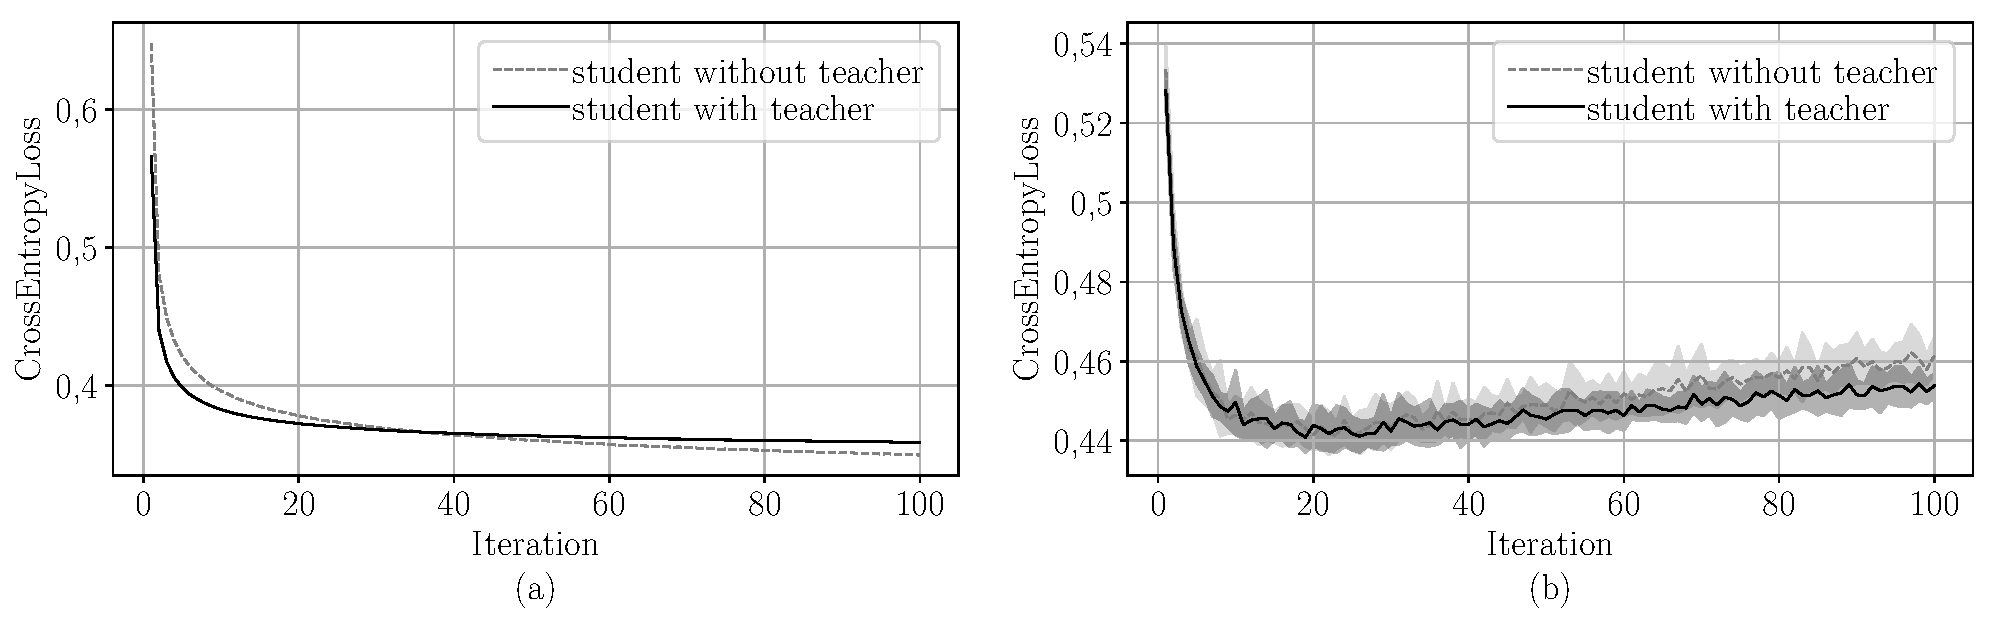
\includegraphics[width=1\textwidth]{figures/mnist_loss}
}

Зависимость кросс--этропии между истинными метками и предсказанными учеников вероятностями классов: a) на обучающей выборке; b) на тестовой выборке.
\end{frame}
%----------------------------------------------------------------------------------------------------------

\begin{frame}{Синтетический эксперимент}
\justifying
Выборка построенная следующим образом:
\[
\begin{aligned}
\mathbf{W} &= \left[\mathcal{N}\bigr(w_{jk}|0, 1\bigr)\right]_{n\times K}, \quad &\mathbf{X} &= \left[\mathcal{N}\bigr(x_{ij}|0, 1\bigr)\right]_{m\times n}, \\
 \mathbf{S} &= \text{softmax}\left(\mathbf{XW}\right), \quad &\mathbf{y} &= \left[\text{Cat}\bigr(y_i| \mathbf{s}_i\bigr)\right],
\end{aligned}
\]
где функция~$\text{softmax}$ берется построчно. Строки матрицы~$\mathbf{S}$ будем рассматривать как предсказание учителя, то есть учитель знает истинные вероятности каждого класса.

В эксперименте число признаков~$n=10$, число классов~$K=3$, для обучения было сгенерировано~$m_{\text{train}}=1000$ и~$m_{\text{test}}=100$ объектов.
\end{frame}
%----------------------------------------------------------------------------------------------------------

\begin{frame}{Синтетический эксперимент: распределение классов}
\justifying
{\center
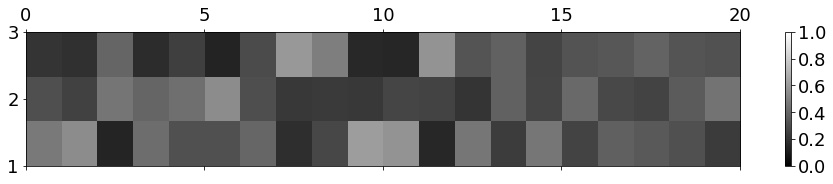
\includegraphics[width=0.9\textwidth]{figures/syn_real_distr}\\
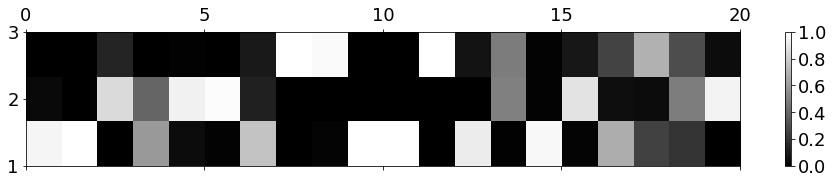
\includegraphics[width=0.9\textwidth]{figures/syn_without_teacher_distr}\\
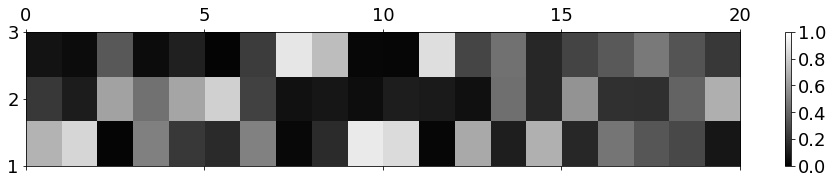
\includegraphics[width=0.9\textwidth]{figures/syn_with_teacher_distr}\\
}
Сверху вниз: истинное распределение; без учителя; с учителем
\end{frame}
%----------------------------------------------------------------------------------------------------------

\begin{frame}{Синтетический эксперимент: анализ параметра $\lambda$ и $T$}
\justifying
{\center
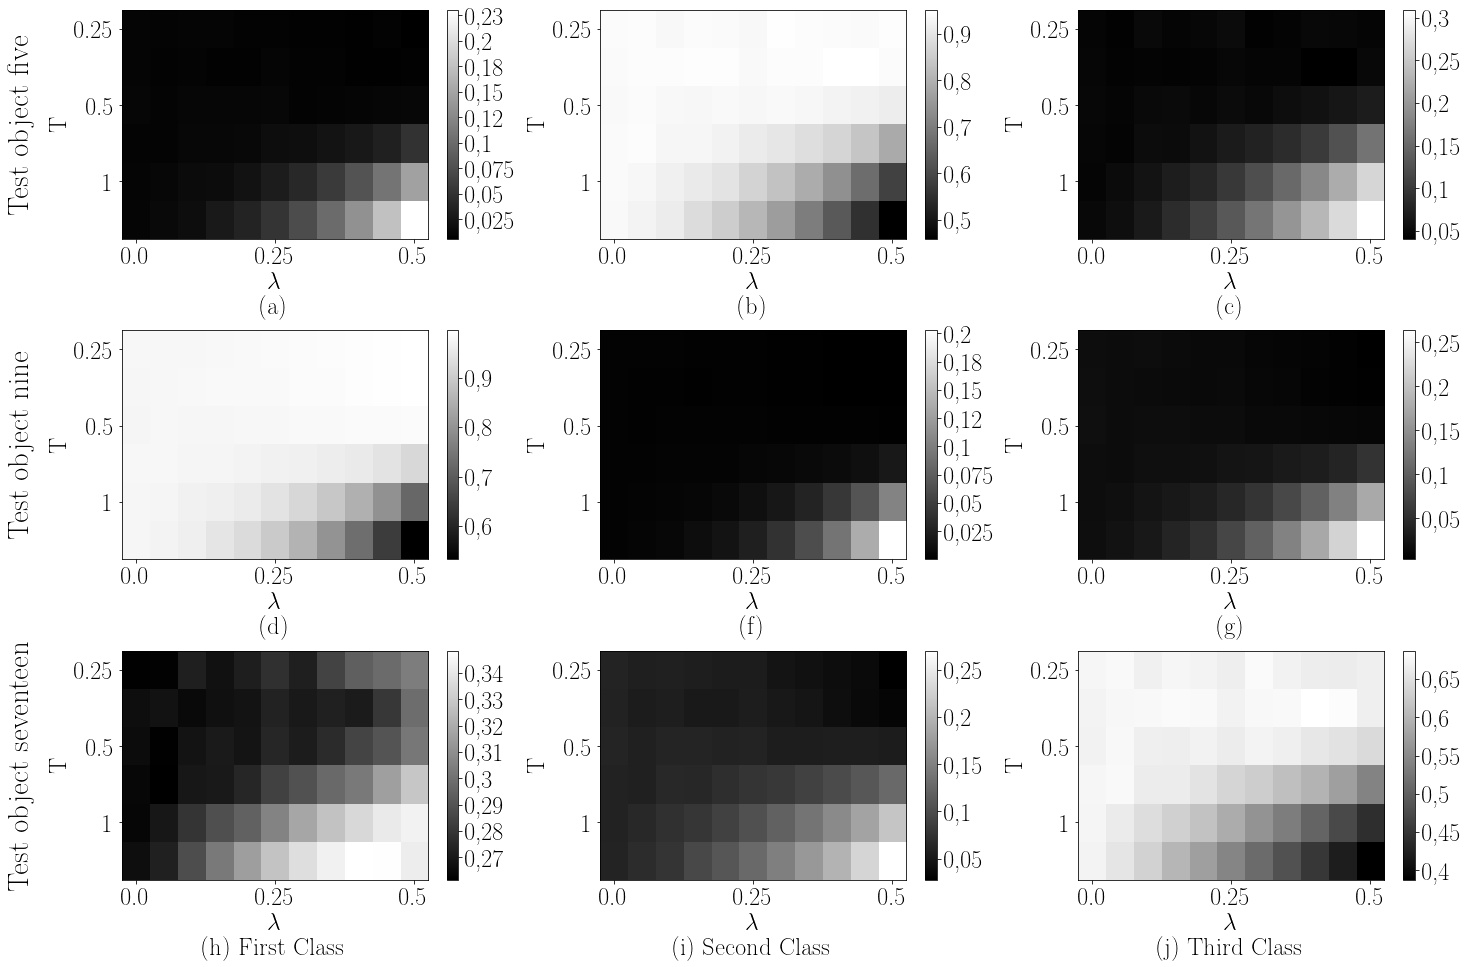
\includegraphics[width=0.9\textwidth]{figures/syn_T_lambda}
}

Зависимость распределения по классам при разных параметрах $\lambda$ и $T$
\end{frame}
%----------------------------------------------------------------------------------------------------------


\begin{frame}{Выборка Twitter Sentiment Analysis}
\justifying
Выборка разделена на~$1{,}18$ миллиона твитов для обучения и~$0{,}35$ миллиона твитов для тестирования. В твитах была выполнена следующая предобработка:
\begin{itemize}
	\item все твиты были переведены в нижний регистр;
	\item все никнеймы вида~``@andrey'' были заменены на токен ``name'';
	\item все цифры были заменены на токен ``number''.
\end{itemize}

~\\
Описание моделей:
\begin{itemize}
	\item модель учителя: модель на основе Bi-LSTM с $\approx 30$ миллионов настраиваемых параметров;
	\item модель ученика: модель на основе предобученной модели BERT с $1538$ настраиваемых параметров.
\end{itemize}

\end{frame}
%----------------------------------------------------------------------------------------------------------


\begin{frame}{Сводная таблица результатов вычислительного эксперимента}
\justifying

\begin{table}[]
\begin{center}
\resizebox{\textwidth}{!}{
	\begin{tabular}{|l|l|c|c|c|}
	\hline
	\multicolumn{1}{|c|}{Dataset} & \multicolumn{1}{c|}{Model} & CrossEntropyLoss      & Accuracy    &   StudentSize   \\ \hline
	\multirow{2}{*}{FashionMnist} & without teacher    &  $0{,}461 \pm 0{,}005$ & $0{,}841\pm 0{,}002$ & 7850 \\ \cline{2-5} 
                              & with teacher       & $0{,}453 \pm 0{,}003$ & $0{,}842 \pm 0{,}002$ & 7850\\ \hline
	\multirow{2}{*}{Synthetic}    & without teacher    & $0{,}225 \pm 0{,}002$ & $0{,}831\pm 0{,}002$ & 33 \\ \cline{2-5} 
                              &  with teacher       & $0{,}452 \pm 0{,}001$   & $0{,}828\pm 0{,}001$ & 33 \\ \hline
	\multirow{2}{*}{Twitter }    & without teacher    & $0{,}501 \pm 0{,}006$ & $0{,}747\pm 0{,}005$ & $1538$  \\ \cline{2-5} 
                              &with teacher       & $0{,}489 \pm 0{,}003$   & $0{,}764\pm 0{,}004$ & $1538$ \\ \hline
	\end{tabular}
}
\end{center}
\end{table}

\end{frame}
%----------------------------------------------------------------------------------------------------------

\begin{frame}{Вывод}
\justifying
Сделано:
	\begin{enumerate}
	\justifying
		\item поставлена вероятностная задача дистилляции моделей глубокого обучения;
		\item проведен теоретический анализ предложенной вероятностной задачи;
		\item проведен вычислительный эксперимент для анализа предложенной модели.
	\end{enumerate}

Планируется:
	\begin{enumerate}
	\justifying
		\item обобщить предложенный метод на случай задачи регрессии более корректно;
		\item использовать байесовский подход выбора моделей машинного обучения для решения данной задачи.
	\end{enumerate}	

\end{frame}
%----------------------------------------------------------------------------------------------------------



\end{document} 